% Options for packages loaded elsewhere
\PassOptionsToPackage{unicode}{hyperref}
\PassOptionsToPackage{hyphens}{url}
%
\documentclass[
  man,floatsintext]{apa6}
\usepackage{amsmath,amssymb}
\usepackage{lmodern}
\usepackage{iftex}
\ifPDFTeX
  \usepackage[T1]{fontenc}
  \usepackage[utf8]{inputenc}
  \usepackage{textcomp} % provide euro and other symbols
\else % if luatex or xetex
  \usepackage{unicode-math}
  \defaultfontfeatures{Scale=MatchLowercase}
  \defaultfontfeatures[\rmfamily]{Ligatures=TeX,Scale=1}
\fi
% Use upquote if available, for straight quotes in verbatim environments
\IfFileExists{upquote.sty}{\usepackage{upquote}}{}
\IfFileExists{microtype.sty}{% use microtype if available
  \usepackage[]{microtype}
  \UseMicrotypeSet[protrusion]{basicmath} % disable protrusion for tt fonts
}{}
\makeatletter
\@ifundefined{KOMAClassName}{% if non-KOMA class
  \IfFileExists{parskip.sty}{%
    \usepackage{parskip}
  }{% else
    \setlength{\parindent}{0pt}
    \setlength{\parskip}{6pt plus 2pt minus 1pt}}
}{% if KOMA class
  \KOMAoptions{parskip=half}}
\makeatother
\usepackage{xcolor}
\IfFileExists{xurl.sty}{\usepackage{xurl}}{} % add URL line breaks if available
\IfFileExists{bookmark.sty}{\usepackage{bookmark}}{\usepackage{hyperref}}
\hypersetup{
  pdftitle={EEG Many Pipelines - Code Mechanics},
  pdfauthor={Sebastian Speer1, Antonio Schettino2,3, \& Ana Martinovici4},
  pdflang={en-EN},
  pdfkeywords={EEG Many Pipelines, scene categorization, vision, EEG, ERP, time-frequency analysis, Bayesian multilevel linear regression, TFCE},
  hidelinks,
  pdfcreator={LaTeX via pandoc}}
\urlstyle{same} % disable monospaced font for URLs
\usepackage{color}
\usepackage{fancyvrb}
\newcommand{\VerbBar}{|}
\newcommand{\VERB}{\Verb[commandchars=\\\{\}]}
\DefineVerbatimEnvironment{Highlighting}{Verbatim}{commandchars=\\\{\}}
% Add ',fontsize=\small' for more characters per line
\usepackage{framed}
\definecolor{shadecolor}{RGB}{248,248,248}
\newenvironment{Shaded}{\begin{snugshade}}{\end{snugshade}}
\newcommand{\AlertTok}[1]{\textcolor[rgb]{0.94,0.16,0.16}{#1}}
\newcommand{\AnnotationTok}[1]{\textcolor[rgb]{0.56,0.35,0.01}{\textbf{\textit{#1}}}}
\newcommand{\AttributeTok}[1]{\textcolor[rgb]{0.77,0.63,0.00}{#1}}
\newcommand{\BaseNTok}[1]{\textcolor[rgb]{0.00,0.00,0.81}{#1}}
\newcommand{\BuiltInTok}[1]{#1}
\newcommand{\CharTok}[1]{\textcolor[rgb]{0.31,0.60,0.02}{#1}}
\newcommand{\CommentTok}[1]{\textcolor[rgb]{0.56,0.35,0.01}{\textit{#1}}}
\newcommand{\CommentVarTok}[1]{\textcolor[rgb]{0.56,0.35,0.01}{\textbf{\textit{#1}}}}
\newcommand{\ConstantTok}[1]{\textcolor[rgb]{0.00,0.00,0.00}{#1}}
\newcommand{\ControlFlowTok}[1]{\textcolor[rgb]{0.13,0.29,0.53}{\textbf{#1}}}
\newcommand{\DataTypeTok}[1]{\textcolor[rgb]{0.13,0.29,0.53}{#1}}
\newcommand{\DecValTok}[1]{\textcolor[rgb]{0.00,0.00,0.81}{#1}}
\newcommand{\DocumentationTok}[1]{\textcolor[rgb]{0.56,0.35,0.01}{\textbf{\textit{#1}}}}
\newcommand{\ErrorTok}[1]{\textcolor[rgb]{0.64,0.00,0.00}{\textbf{#1}}}
\newcommand{\ExtensionTok}[1]{#1}
\newcommand{\FloatTok}[1]{\textcolor[rgb]{0.00,0.00,0.81}{#1}}
\newcommand{\FunctionTok}[1]{\textcolor[rgb]{0.00,0.00,0.00}{#1}}
\newcommand{\ImportTok}[1]{#1}
\newcommand{\InformationTok}[1]{\textcolor[rgb]{0.56,0.35,0.01}{\textbf{\textit{#1}}}}
\newcommand{\KeywordTok}[1]{\textcolor[rgb]{0.13,0.29,0.53}{\textbf{#1}}}
\newcommand{\NormalTok}[1]{#1}
\newcommand{\OperatorTok}[1]{\textcolor[rgb]{0.81,0.36,0.00}{\textbf{#1}}}
\newcommand{\OtherTok}[1]{\textcolor[rgb]{0.56,0.35,0.01}{#1}}
\newcommand{\PreprocessorTok}[1]{\textcolor[rgb]{0.56,0.35,0.01}{\textit{#1}}}
\newcommand{\RegionMarkerTok}[1]{#1}
\newcommand{\SpecialCharTok}[1]{\textcolor[rgb]{0.00,0.00,0.00}{#1}}
\newcommand{\SpecialStringTok}[1]{\textcolor[rgb]{0.31,0.60,0.02}{#1}}
\newcommand{\StringTok}[1]{\textcolor[rgb]{0.31,0.60,0.02}{#1}}
\newcommand{\VariableTok}[1]{\textcolor[rgb]{0.00,0.00,0.00}{#1}}
\newcommand{\VerbatimStringTok}[1]{\textcolor[rgb]{0.31,0.60,0.02}{#1}}
\newcommand{\WarningTok}[1]{\textcolor[rgb]{0.56,0.35,0.01}{\textbf{\textit{#1}}}}
\usepackage{graphicx}
\makeatletter
\def\maxwidth{\ifdim\Gin@nat@width>\linewidth\linewidth\else\Gin@nat@width\fi}
\def\maxheight{\ifdim\Gin@nat@height>\textheight\textheight\else\Gin@nat@height\fi}
\makeatother
% Scale images if necessary, so that they will not overflow the page
% margins by default, and it is still possible to overwrite the defaults
% using explicit options in \includegraphics[width, height, ...]{}
\setkeys{Gin}{width=\maxwidth,height=\maxheight,keepaspectratio}
% Set default figure placement to htbp
\makeatletter
\def\fps@figure{htbp}
\makeatother
\setlength{\emergencystretch}{3em} % prevent overfull lines
\providecommand{\tightlist}{%
  \setlength{\itemsep}{0pt}\setlength{\parskip}{0pt}}
\setcounter{secnumdepth}{5}
% Make \paragraph and \subparagraph free-standing
\ifx\paragraph\undefined\else
  \let\oldparagraph\paragraph
  \renewcommand{\paragraph}[1]{\oldparagraph{#1}\mbox{}}
\fi
\ifx\subparagraph\undefined\else
  \let\oldsubparagraph\subparagraph
  \renewcommand{\subparagraph}[1]{\oldsubparagraph{#1}\mbox{}}
\fi
\newlength{\cslhangindent}
\setlength{\cslhangindent}{1.5em}
\newlength{\csllabelwidth}
\setlength{\csllabelwidth}{3em}
\newlength{\cslentryspacingunit} % times entry-spacing
\setlength{\cslentryspacingunit}{\parskip}
\newenvironment{CSLReferences}[2] % #1 hanging-ident, #2 entry spacing
 {% don't indent paragraphs
  \setlength{\parindent}{0pt}
  % turn on hanging indent if param 1 is 1
  \ifodd #1
  \let\oldpar\par
  \def\par{\hangindent=\cslhangindent\oldpar}
  \fi
  % set entry spacing
  \setlength{\parskip}{#2\cslentryspacingunit}
 }%
 {}
\usepackage{calc}
\newcommand{\CSLBlock}[1]{#1\hfill\break}
\newcommand{\CSLLeftMargin}[1]{\parbox[t]{\csllabelwidth}{#1}}
\newcommand{\CSLRightInline}[1]{\parbox[t]{\linewidth - \csllabelwidth}{#1}\break}
\newcommand{\CSLIndent}[1]{\hspace{\cslhangindent}#1}
\ifLuaTeX
\usepackage[bidi=basic]{babel}
\else
\usepackage[bidi=default]{babel}
\fi
\babelprovide[main,import]{english}
% get rid of language-specific shorthands (see #6817):
\let\LanguageShortHands\languageshorthands
\def\languageshorthands#1{}
% Manuscript styling
\usepackage{upgreek}
\captionsetup{font=singlespacing,justification=justified}

% Table formatting
\usepackage{longtable}
\usepackage{lscape}
% \usepackage[counterclockwise]{rotating}   % Landscape page setup for large tables
\usepackage{multirow}		% Table styling
\usepackage{tabularx}		% Control Column width
\usepackage[flushleft]{threeparttable}	% Allows for three part tables with a specified notes section
\usepackage{threeparttablex}            % Lets threeparttable work with longtable

% Create new environments so endfloat can handle them
% \newenvironment{ltable}
%   {\begin{landscape}\centering\begin{threeparttable}}
%   {\end{threeparttable}\end{landscape}}
\newenvironment{lltable}{\begin{landscape}\centering\begin{ThreePartTable}}{\end{ThreePartTable}\end{landscape}}

% Enables adjusting longtable caption width to table width
% Solution found at http://golatex.de/longtable-mit-caption-so-breit-wie-die-tabelle-t15767.html
\makeatletter
\newcommand\LastLTentrywidth{1em}
\newlength\longtablewidth
\setlength{\longtablewidth}{1in}
\newcommand{\getlongtablewidth}{\begingroup \ifcsname LT@\roman{LT@tables}\endcsname \global\longtablewidth=0pt \renewcommand{\LT@entry}[2]{\global\advance\longtablewidth by ##2\relax\gdef\LastLTentrywidth{##2}}\@nameuse{LT@\roman{LT@tables}} \fi \endgroup}

% \setlength{\parindent}{0.5in}
% \setlength{\parskip}{0pt plus 0pt minus 0pt}

% Overwrite redefinition of paragraph and subparagraph by the default LaTeX template
% See https://github.com/crsh/papaja/issues/292
\makeatletter
\renewcommand{\paragraph}{\@startsection{paragraph}{4}{\parindent}%
  {0\baselineskip \@plus 0.2ex \@minus 0.2ex}%
  {-1em}%
  {\normalfont\normalsize\bfseries\itshape\typesectitle}}

\renewcommand{\subparagraph}[1]{\@startsection{subparagraph}{5}{1em}%
  {0\baselineskip \@plus 0.2ex \@minus 0.2ex}%
  {-\z@\relax}%
  {\normalfont\normalsize\itshape\hspace{\parindent}{#1}\textit{\addperi}}{\relax}}
\makeatother

% \usepackage{etoolbox}
\makeatletter
\patchcmd{\HyOrg@maketitle}
  {\section{\normalfont\normalsize\abstractname}}
  {\section*{\normalfont\normalsize\abstractname}}
  {}{\typeout{Failed to patch abstract.}}
\patchcmd{\HyOrg@maketitle}
  {\section{\protect\normalfont{\@title}}}
  {\section*{\protect\normalfont{\@title}}}
  {}{\typeout{Failed to patch title.}}
\makeatother

\usepackage{xpatch}
\makeatletter
\xapptocmd\appendix
  {\xapptocmd\section
    {\addcontentsline{toc}{section}{\appendixname\ifoneappendix\else~\theappendix\fi\\: #1}}
    {}{\InnerPatchFailed}%
  }
{}{\PatchFailed}
\keywords{EEG Many Pipelines, scene categorization, vision, EEG, ERP, time-frequency analysis, Bayesian multilevel linear regression, TFCE\newline\indent Word count: X}
\usepackage{csquotes}
\ifLuaTeX
  \usepackage{selnolig}  % disable illegal ligatures
\fi

\title{EEG Many Pipelines - Code Mechanics}
\author{Sebastian Speer\textsuperscript{1}, Antonio Schettino\textsuperscript{2,3}, \& Ana Martinovici\textsuperscript{4}}
\date{}


\shorttitle{Code Mechanics}

\authornote{

Authorship order was randomly determined via the \texttt{sample} function in \emph{R}.

\textbf{SS} preprocessed the data and performed time-frequency analysis (research questions 2b, 2c, 3b, 4b). \textbf{AS} preprocessed the data and performed ERP analysis (research questions 1, 2a, 3a, 4a). \textbf{AM} was responsible for project management, GitHub repository, and reproducibility. \textbf{SS}, \textbf{AS}, and \textbf{AM} wrote the report.

Correspondence concerning this article should be addressed to Ana Martinovici, Burgemeester Oudlaan 50, 3062 PA Rotterdam, Netherlands. E-mail: \href{mailto:martinovici@rsm.nl}{\nolinkurl{martinovici@rsm.nl}}

}

\affiliation{\vspace{0.5cm}\textsuperscript{1} Social Brain Lab, Netherlands Institute for Neuroscience, Amsterdam, The Netherlands\\\textsuperscript{2} Erasmus Research Services, Erasmus University Rotterdam, Rotterdam, The Netherlands\\\textsuperscript{3} Institute for Globally Distributed Open Research and Education (IGDORE), Sweden\\\textsuperscript{4} Rotterdam School or Management, Erasmus University Rotterdam, Rotterdam, The Netherlands}

\abstract{%
One or two sentences providing a \textbf{basic introduction} to the field, comprehensible to a scientist in any discipline.

Two to three sentences of \textbf{more detailed background}, comprehensible to scientists in related disciplines.

One sentence clearly stating the \textbf{general problem} being addressed by this particular study.

One sentence summarizing the main result (with the words ``\textbf{here we show}'' or their equivalent).

Two or three sentences explaining what the \textbf{main result} reveals in direct comparison to what was thought to be the case previously, or how the main result adds to previous knowledge.

One or two sentences to put the results into a more \textbf{general context}.

Two or three sentences to provide a \textbf{broader perspective}, readily comprehensible to a scientist in any discipline.
}



\begin{document}
\maketitle

\hypertarget{introduction}{%
\section{Introduction}\label{introduction}}

Timeline of our contribution to the EEGManyPipelines project:

\begin{itemize}
\item
  we registered for the EEGManyPipelines project on 2021-09-15, and received the confirmation email 2021-09-20.
\item
  instructions for downloading the data and for analysis were sent 2021-10-08. These are saved within the repository at \texttt{data\_in\_repo/original\_data/instructions}.
\item
  we received the link to the submission portal on 2022-05-02
\item
  we've submitted the pre-processed data on
\end{itemize}

\hypertarget{methods}{%
\section{Methods}\label{methods}}

\hypertarget{preprocessing---erp}{%
\subsection{Preprocessing - ERP}\label{preprocessing---erp}}

The continuous EEG data was assigned electrode coordinates and filtered with two consecutive Hamming windowed sinc FIR filters (high-pass 0.1 Hz, low-pass 40 Hz). Bad or noisy channels were detected using several approaches implemented in the PREP pipeline (\protect\hyperlink{ref-bigdely-shamlo2015}{Bigdely-Shamlo, Mullen, Kothe, Su, \& Robbins, 2015}), including flat or missing signal, ``bad-by-high-frequency-noise'' (frequency components above 50 Hz considerably higher than median channel noisiness, as calculated using a robust \emph{Z}-scoring method and default threshold \emph{z} \textgreater{} 5), ``bad-by-correlation'' (maximum correlation with another channel below the default \emph{r} = .4; fraction of bad correlation windows above the default threshold of 0.01), ``bad-by-deviation'' (amplitude deviates from the median channel amplitude, as calculated using a robust \emph{Z}-scoring method and default threshold \emph{z} \textgreater{} 5), and signal prediction based on signals and spatial locations of other channels lower than default threshold of \emph{r} = .75 (random sample consensus approach, RANSAC; Fischler and Bolles (\protect\hyperlink{ref-fischler1987}{1987})).\footnote{For more details, see the documentation of \href{https://pyprep.readthedocs.io/en/latest/generated/pyprep.NoisyChannels.html\#pyprep.NoisyChannels}{pyprep.NoisyChannels}.}\\

First, by means of correlation, we checked how well a given channel is correlated with all other channels (categorized as bad at \emph{r} , 0.4); second, we checked by using the robust \emph{z}-score deviation aggregates per channel (categorized as bad at \emph{z} . 5); third, by using the robust \emph{z}-score estimates of high-frequency noise per channel (categorized as bad at \emph{z} . 5); and finally, we checked by using the random sample consensus (RANSAC) channel correlations, which is the correlation for each channel with itself across the original data versus the RANSAC predicted data (categorized as bad at \emph{r} , 0.75) as implemented in the PREP pipeline (\protect\hyperlink{ref-bigdely-shamlo2015}{Bigdely-Shamlo et al., 2015}). After detection, these channels were removed from the data and subsequently interpolated (i.e., estimated from surrounding channels). Interpolation was performed using the spherical spline method (\protect\hyperlink{ref-perrin1989}{Perrin, Pernier, Bertrand, \& Echallier, 1989}) as implemented in MNE-Python, which projects the sensor locations onto a unit sphere and interpolates the signal at the channels identified as bad on the signals for the good channels.

Noisy channels were interpolated via a spherical spline procedure82. Please note that the interpolated channels were mostly identifed outside of the clusters selected for the ERP components defnition (max interpolated channels in clusters: (2); therefore, any potential distortions of the EEG signal due to interpolation was negligible. Ocular channels were discarded, and the scalp data re-referenced to the average signal. Epochs extending from −200ms to +1,000ms time-locked to word onset were created, and baseline correction was applied using the pre-stimulus interval. Finally, 8 grand-averages were computed following each combination of our 2×2×2 factorial design: (1) negative words, large font, high contrast; (2) negative words, small font, high contrast; (3) negative words, large font, low contrast; (4) negative words, small font, low contrast; (5) neutral words, large font, high contrast; (6) neutral words, small font, high contrast; (7) neutral words, large font, low contrast; (8) neutral words, small font, low contrast. Identifcation of ERP components

\hypertarget{preprocessing---tfr}{%
\subsection{Preprocessing - TFR}\label{preprocessing---tfr}}

EEG data were filtered with a low cutoff filter of 1 Hz to remove slow drifts, a high cutoff filter at 40 Hz to attenuate high frequency power. Subsequently, bad and noisy channels were detected using several different approaches as implemented in the PREP pipeline (\protect\hyperlink{ref-bigdely-shamlo2015}{Bigdely-Shamlo et al., 2015}). First, by means of correlation, we checked how well a given channel is correlated with all other channels (categorized as bad at \emph{r} , 0.4); second, we checked by using the robust \emph{z}-score deviation aggregates per channel (categorized as bad at \emph{z} . 5); third, by using the robust \emph{z}-score estimates of high-frequency noise per channel (categorized as bad at \emph{z} . 5); and finally, we checked by using the random sample consensus (RANSAC) channel correlations, which is the correlation for each channel with itself across the original data versus the RANSAC predicted data (categorized as bad at \emph{r} , 0.75) as implemented in the PREP pipeline (\protect\hyperlink{ref-bigdely-shamlo2015}{Bigdely-Shamlo et al., 2015}). After detection, these channels were removed from the data and subsequently interpolated (i.e., estimated from surrounding channels). Interpolation was performed using the spherical spline method (\protect\hyperlink{ref-perrin1989}{Perrin et al., 1989}) as implemented in MNE-Python, which projects the sensor locations onto a unit sphere and interpolates the signal at the channels identified as bad on the signals for the good channels. Afterwards, the EEG data were re-referenced to the average signal across channels. Next, ocular artifacts were removed by performing an independent component analysis on the data and then correlating the resulting components with the EOG channels to see which of the components represented the ocular artifacts. The component that correlated the highest with the EOG channels was then removed from the EEG data.

add: \url{https://pyprep.readthedocs.io/en/stable/generated/pyprep.NoisyChannels.html\#pyprep.NoisyChannels}

\hypertarget{cutoffs}{%
\subsubsection{Cutoffs}\label{cutoffs}}

Implemented in file: /code\_mechanics/scripts/TFR\_preproc\_step1.py, lines 30:32.

\begin{Shaded}
\begin{Highlighting}[]
    \CommentTok{\# filter cutoffs}
\NormalTok{    cutoff\_low }\OtherTok{=} \DecValTok{1} \CommentTok{\# adapated to TFR analysis}
\NormalTok{    cutoff\_high }\OtherTok{=} \DecValTok{40}
\end{Highlighting}
\end{Shaded}

\hypertarget{bad-channels-at-0.4}{%
\subsubsection{Bad Channels at 0.4}\label{bad-channels-at-0.4}}

Implemented in file: /code\_mechanics/scripts/TFR\_preproc\_step1.py, lines 279:298.

\begin{Shaded}
\begin{Highlighting}[]
        \CommentTok{\# detect noisy channels based on:}
        \CommentTok{\# {-} missing signal (NaN)}
        \CommentTok{\# {-} flat signal}
        \CommentTok{\# {-} deviation}
        \CommentTok{\# {-} HF noise (frequency components \textgreater{} 50 Hz considerably higher than median channel noisiness)}
        \CommentTok{\# {-} correlation}
        \CommentTok{\#   {-} bad correlation window if maximum correlation with another channel is below the provided correlation threshold (default: 0.4)}
        \CommentTok{\#   {-} a channel is “bad{-}by{-}correlation” if its fraction of bad correlation windows is above the bad fraction threshold (default: 0.01)}
        \CommentTok{\# {-} low signal{-}to{-}noise ratio (too much high{-}frequency noise + low channel correlation)}
        \CommentTok{\# {-} dropout (long time windows with completely flat signal, default fraction threshold 0.01)}
        \CommentTok{\# {-} RANSAC (random sample consensus approach): predict signal based on signals and spatial locations of other currently{-}good channels}
        \CommentTok{\#   {-} split recording into non{-}overlapping time windows (default: 5 seconds)}
        \CommentTok{\#   {-} correlate each channel’s RANSAC{-}predicted signal with its actual signal}
        \CommentTok{\#   {-} bad window if predicted vs. actual signal correlation below correlation threshold (default: 0.75)}
        \CommentTok{\#   {-} bad channel if its fraction of bad RANSAC windows is above threshold (default: 0.4)}
        \CommentTok{\# for more info, see https://pyprep.readthedocs.io/en/latest/generated/pyprep.NoisyChannels.html\#pyprep.NoisyChannels}
        \FunctionTok{nd.find\_all\_bads}\NormalTok{(}
            \AttributeTok{ransac =}\NormalTok{ True, }
            \AttributeTok{channel\_wise =}\NormalTok{ False}
\NormalTok{            )}
\end{Highlighting}
\end{Shaded}

\hypertarget{questions-for-sebastian}{%
\subsubsection{Questions for Sebastian}\label{questions-for-sebastian}}

\begin{itemize}
\tightlist
\item
  Where do you check the ``robust \emph{z}-score deviation aggregates per channel (categorized as bad at \emph{z} . 5)''?
\end{itemize}

This is in the default setting of the function.

\begin{itemize}
\tightlist
\item
  Is the ``do not apply 1 Hz high-pass filter'' comment accurate? If so, isn't that what happens at lines 242:247?
\end{itemize}

the comments from lines 272:274 can and should be deleted

Implemented in file: /code\_mechanics/scripts/TFR\_preproc\_step1.py, lines 241:247.

\begin{Shaded}
\begin{Highlighting}[]
        \CommentTok{\# filter data}
\NormalTok{        raw }\OtherTok{=} \FunctionTok{raw.filter}\NormalTok{( }\CommentTok{\# apply high{-}pass filter}
            \AttributeTok{l\_freq =}\NormalTok{ cutoff\_low,}
            \AttributeTok{h\_freq =}\NormalTok{ None)}\FunctionTok{.filter}\NormalTok{( }\CommentTok{\# apply low{-}pass filter}
                \AttributeTok{l\_freq =}\NormalTok{ None,}
                \AttributeTok{h\_freq =}\NormalTok{ cutoff\_high}
\NormalTok{                )}
\end{Highlighting}
\end{Shaded}

Implemented in file: /code\_mechanics/scripts/TFR\_preproc\_step1.py, lines 269:277.

\begin{Shaded}
\begin{Highlighting}[]
        \CommentTok{\# detect noisy channels}
\NormalTok{        nd }\OtherTok{=} \FunctionTok{NoisyChannels}\NormalTok{(}
\NormalTok{            raw,}
            \CommentTok{\# do not apply 1 Hz high{-}pass filter before bad channel detection:}
            \CommentTok{\# the data have already been high{-}pass filtered at 0.1 Hz}
            \CommentTok{\# and we don\textquotesingle{}t want to miss bad channels with slow drifts}
            \AttributeTok{do\_detrend =}\NormalTok{ False,}
            \AttributeTok{random\_state =}\NormalTok{ project\_seed }\CommentTok{\# RNG seed}
\NormalTok{            )}
\end{Highlighting}
\end{Shaded}

\hypertarget{epoching}{%
\subsection{Epoching}\label{epoching}}

The EEG data was then subsampled by a factor of four (i.e., from 512 Hz to 128 Hz and segmented into 800 ms epochs, with 300 ms before stimulus onset (onset of the scene) until 500 ms after stimulus onset. The epochs were baseline corrected using the 300 ms preceding the stimulus onset. The resulting epochs were then subjected to \emph{Autoreject}, an automated artifact detection algorithm based on machine-learning classifiers, and cross-validation to estimate the optimal peak-to-peak threshold (\protect\hyperlink{ref-jas2017}{Jas, Engemann, Bekhti, Raimondo, \& Gramfort, 2017}). This algorithm was implemented to remove artifacts not identified by previous preprocessing steps, and depending on the number of bad sensors for a given trial, either repairs the trial based on interpolation or excludes it from further analysis. The preprocessed data were then submitted to a Morlet wavelet analysis to transform the data into the time-frequency domain with 18 log-scaled frequency bins ranging from 4 to 40 Hz to have higher sensitivity in lower frequency ranges such as the theta band. To optimize both spectral and temporal resolution, the number of cycles to include in the sliding time window were defined by dividing each individual frequency by two. After transforming the data to the time-frequency domain, the data were decimated by a factor of two (sampling every second time point) to increase computational efficiency.

\hypertarget{downsample-and-segmentation}{%
\subsubsection{downsample and segmentation}\label{downsample-and-segmentation}}

Implemented in file: /code\_mechanics/scripts/TFR\_preproc\_step1.py, lines 413:427.

\begin{Shaded}
\begin{Highlighting}[]
        \CommentTok{\# create epochs (all conditions)}
        \CommentTok{\# }\AlertTok{NOTE}\CommentTok{: epochs are subsampled (512 Hz {-}{-}\textgreater{} 128 Hz),}
        \CommentTok{\# to lower the chances of Type II error in subsequent statistical analyses}
\NormalTok{        epochs }\OtherTok{=} \FunctionTok{mne.Epochs}\NormalTok{(}
\NormalTok{            raw, }
\NormalTok{            events, }\CommentTok{\# events}
            \AttributeTok{tmin =}\NormalTok{ begin\_epoch, }\CommentTok{\# start epoch}
            \AttributeTok{tmax =}\NormalTok{ end\_epoch, }\CommentTok{\#end epoch}
            \AttributeTok{baseline =}\NormalTok{ (begin\_epoch, }\DecValTok{0}\NormalTok{), }\CommentTok{\# time window for baseline correction}
            \AttributeTok{picks =}\NormalTok{ None, }\CommentTok{\# include all channels }
            \AttributeTok{preload =}\NormalTok{ True,}
            \AttributeTok{decim =} \DecValTok{4}\NormalTok{, }\CommentTok{\# subsample data by a factor of 4, i.e., 128 Hz (for more info, see https://mne.tools/stable/overview/faq.html\#resampling{-}and{-}decimating)}
            \AttributeTok{detrend =}\NormalTok{ None, }\CommentTok{\# do not detrend before baseline correction        }
            \AttributeTok{reject\_by\_annotation =}\NormalTok{ False }\CommentTok{\# do not reject based on annotations}
\NormalTok{            )}
\end{Highlighting}
\end{Shaded}

\hypertarget{analysis}{%
\section{Analysis}\label{analysis}}

\hypertarget{rq1}{%
\subsection{RQ1}\label{rq1}}

The first hypothesis we were asked to test was the following:

\begin{quote}
\emph{There is an effect of scene category (i.e., a difference between images showing man-made vs.~natural environments) on the amplitude of the N1 component, i.e.~the first major negative EEG voltage deflection.}
\end{quote}

To address this question, we fit a Bayesian multilevel linear model on N1 amplitude values, with \emph{condition} (2 levels: \emph{man-made}, \emph{natural}) as \emph{constant} (a.k.a. fixed) effect and participant and trial as \emph{varying} (a.k.a. random) effects. We allowed intercepts and slopes to vary as a function of participant and trials, to model general and condition-specific inter-individual differences. As a likelihood function, we chose a Gaussian distribution.\\
An important aspect of Bayesian analysis is the choice of priors (e.g., \protect\hyperlink{ref-natarajan2000}{Natarajan \& Kass, 2000}). Given the susceptibility of the electrophysiological signal to inter-individual differences (e.g., skull thickness, skin conductance, or hair), we decided to base our priors on the current data by visually inspecting the grand average ERP waveform, i.e., collapsed across \emph{man-made} and \emph{natural} condition. This procedure follows the same logic of \emph{collapsed localizers}, useful when prior research does not allow to reliably identify scalp electrodes and time windows related to ERP components of interest (e.g., \protect\hyperlink{ref-Luck2017}{Luck \& Gaspelin, 2017, p. 150}). For the main analysis, we placed \textbf{informative priors} on the \emph{intercept} -- a normal distribution with mean \(\mu\) = 4 and standard deviation \(\sigma\) = 2: \(Normal(4,2)\) -- and \(\beta\) coefficient, \(Normal(0,1)\). To assess whether our chosen informative prior would bias parameter estimates (and, consequently, the interpretation of the results; Depaoli and van de Schoot (\protect\hyperlink{ref-depaoli2017}{2017})), we ran the same multilevel linear model with \textbf{weakly informative} priors (\emph{intercept}: \(Normal(4,4)\) ; \(\beta\): \(Normal(0,4)\)) and \textbf{uninformative} priors (\emph{intercept}: \(Normal(4,10)\) ; \(\beta\): \(Normal(0,10)\)). We anticipated that the choice of prior would have negligible effects on the posterior distributions, because the influence of the prior washes out with a large amount of data (\protect\hyperlink{ref-edwards1963}{Edwards, Lindman, \& Savage, 1963}).\\
Since we had no prior knowledge regarding the standard deviation of participant and trials, we placed a \textbf{weakly informative prior} on these varying effects: a \emph{t}-distribution with degrees of freedom \(\nu\) = 3, location \(\mu\) = 0, and scale \(\sigma\) = 2, \(Student(3,0,2)\).\\
Models were fitted in \emph{R} using the \texttt{brms} package (\protect\hyperlink{ref-buxfcrkner2018}{Bürkner, 2018}), which employs the probabilistic programming language \emph{Stan} (\protect\hyperlink{ref-carpenter2017}{Carpenter et al., 2017}) to implement a Markov chain Monte Carlo (MCMC) algorithm (i.e., No-U-Turn sampler; Homan and Gelman (\protect\hyperlink{ref-homan2014}{2014})) to estimate posterior distributions of the parameters of interest. Four MCMC chains with 4000 iterations (2000 warm-up) and no thinning were run to estimate parameters in each of the fitted models. Model convergence was assessed as follows: (\emph{i}) visual inspection of trace plots, rank plots, and graphical posterior predictive checks (\protect\hyperlink{ref-gabry2019}{Gabry, Simpson, Vehtari, Betancourt, \& Gelman, 2019}); (\emph{ii}) Gelman-Rubin \(\hat{R}\) statistic (\protect\hyperlink{ref-gelman2013}{Gelman et al., 2013}) -- comparing the between-chains variability to the within-chain variability -- between 1 and 1.05 (see also \protect\hyperlink{ref-Nalborczyk2019}{Nalborczyk, Batailler, Lœvenbruck, Vilain, \& Bürkner, 2019}).\\
Posterior distributions of the model parameters were summarized using the mean and 95\% credible interval (CI). Differences between conditions were calculated by computing the difference between posterior distributions of the respective conditions.\\
Statistical inference was performed using the \textbf{HDI + ROPE} decision rule (\protect\hyperlink{ref-kruschke2018}{Kruschke, 2018}): values were accepted or rejected against a null hypothesis considering a small effect as practically equivalent to zero (Region of Practical Equivalence; \emph{ROPE}). To mitigate the inevitable subjectivity intrinsic in arbitrarily choosing the range of negligible values, we explored a range of plausible ROPEs, from ±0.05\(\mu\)\emph{V} to ±0.5\(\mu\)\emph{V} in steps of 0.01\(\mu\)\emph{V}. If the percentage of the posterior differences within the full ROPE was smaller than 5\%, the null hypothesis was rejected.

\hypertarget{add-scoring-of-n1}{%
\subsubsection{ADD SCORING OF N1}\label{add-scoring-of-n1}}

\hypertarget{rq2}{%
\subsection{RQ2}\label{rq2}}

To test whether there are effects of image novelty (RQ2; i.e., between images shown for the first time/new vs.~repeated/old images) we conducted a multilevel analysis contrasting the EEG data from trials with old images against trials with new images. To test for differences in theta power at fronto-central channels we focused on the frequency range from 4-8 Hz and all frontocentral channels (FC1, FCz, FC2). At the first level (i.e., the participant level), we computed the averaged time-frequency maps for each of the two conditions. We then tested the resulting averaged maps at the second level for significant group effects, using a paired-sample \emph{t}-test. We used cluster-based permutation testing as a stringent control for multiple comparisons (\protect\hyperlink{ref-maris2007}{Maris \& Oostenveld, 2007}). Specifically, for every sample across the three channels, we quantified the experimental effect by a \emph{t} value. Selection of samples for inclusion in a cluster was implemented using threshold-free cluster enhancement (TFCE) (\protect\hyperlink{ref-smith2009}{Smith \& Nichols, 2009}). TFCE eliminates the free parameter initial threshold value that determines which points are included in clustering by approximating a continuous integration across possible threshold values with a standard Riemann sum. We subsequently clustered selected samples in connected sets based on temporal and spectral adjacency, and we computed cluster-level statistics by taking the sum of the \emph{t} values within every cluster. Subsequently, we performed permutation testing using the Monte Carlo method to compute the posterior significance probability of our observed effect(\protect\hyperlink{ref-maris2007}{Maris \& Oostenveld, 2007}). This analysis results in a cluster of adjacent data points across time, frequencies, and channels, which significantly differs in activity between old and new images. To test for differences in alpha power at posterior channels we focused on the frequency range from 8-13 Hz and all posterior channels (P7, P5, P3, P1, P2, P4, P6).

\hypertarget{questions}{%
\subsubsection{Questions}\label{questions}}

Do we need to use adjency? We have that in RQ3 ERP, but not TFR: \url{https://mne.tools/stable/generated/mne.stats.permutation_cluster_test.html?highlight=permutation_cluster_test\#mne.stats.permutation_cluster_test}

\hypertarget{rq3}{%
\subsection{RQ3}\label{rq3}}

The same analysis approach as described for RQ2 was implemented for RQ3. Specifically, to test whether there are effects of successful recognition of old images on spectral power, at any frequencies, at any channel, at any time, we contrasted time-frequency decomposed EEG data from trials containing old images that were correctly recognized as old with old images incorrectly recognized as new. Here we included all frequencies, timepoints, and channels in the analysis. The same thresholding procedure and permutation testing approach as above was used.

\hypertarget{rq4}{%
\subsection{RQ4}\label{rq4}}

To test whether there are effects of subsequent memory, we conducted exactly the same analysis as described in RQ3, with the only difference that here we contrasted trial containing images that will be successfully remembered vs.~forgotten on a subsequent repetition.

\hypertarget{results}{%
\section{Results}\label{results}}



\begin{figure}
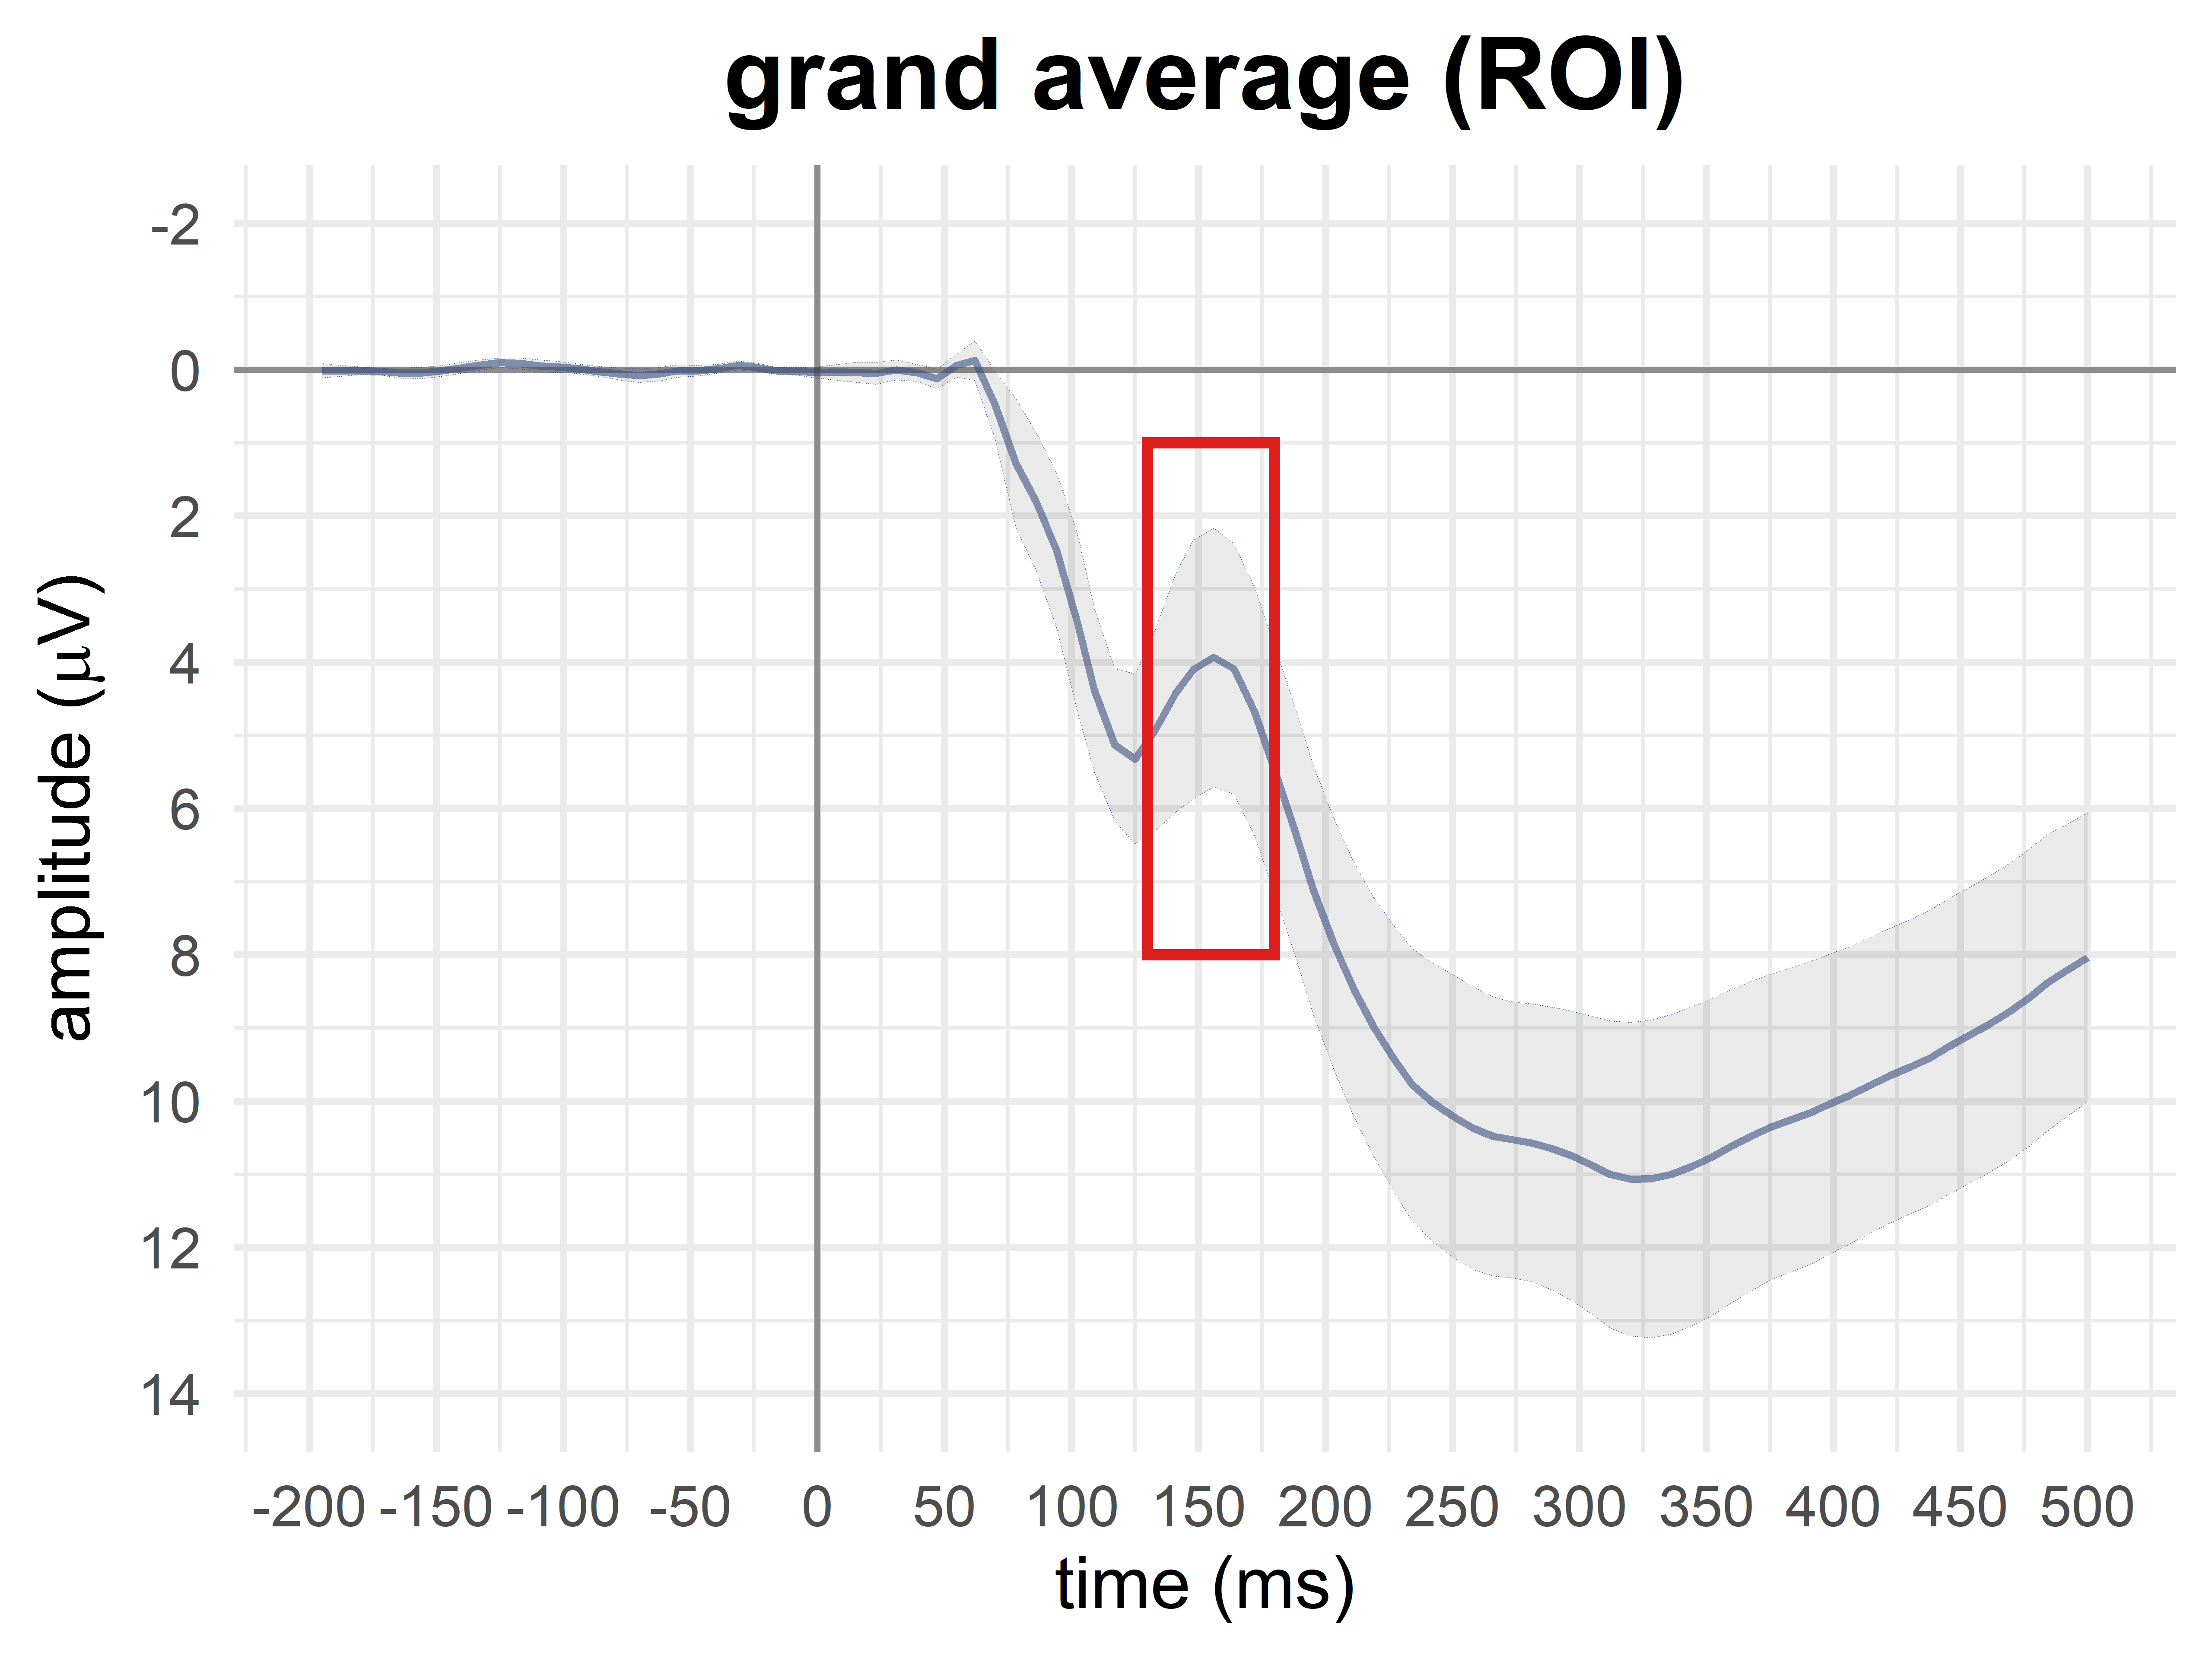
\includegraphics[width=0.9\linewidth]{../results_in_repo/RQ1/timeseries_grand_average_ROI} \caption{My caption.}\label{fig:figure01}
\end{figure}

No significant clusters were identified for any of the research questions (at \(\alpha\) = 0.05).

\hypertarget{discussion}{%
\section{Discussion}\label{discussion}}

ADD DISCUSSION HERE

\hypertarget{software}{%
\section{Software}\label{software}}

EEG preprocessing was carried out using \texttt{MNE-Python} (\protect\hyperlink{ref-gramfort2013}{Gramfort, 2013}) in \emph{Python} \emph{v}3.9.7 (\protect\hyperlink{ref-vanrossum-2009}{Van Rossum \& Drake, 2009}) and \emph{Spyder IDE} \emph{v}5.1.5 (\protect\hyperlink{ref-raybaut2009}{Raybaut, 2009}). Analysis, visualization, and report generation were carried out in \emph{R} \emph{v}4.1.3 (\protect\hyperlink{ref-R-base}{R Core Team, 2022}) and \emph{RStudio IDE} \emph{v}2022.02.1+461 (\protect\hyperlink{ref-R-studio}{RStudio Team, 2020}). We used the following \emph{R} packages:

\begin{itemize}
\item
  \textbf{data wrangling and analysis}: \texttt{here} \emph{v}1.0.1 (\protect\hyperlink{ref-here}{Müller, 2020}), \texttt{Rmisc} \emph{v}1.5 (\protect\hyperlink{ref-Rmisc}{Hope, 2022}), \texttt{tidyverse} \emph{v}1.3.1 (\protect\hyperlink{ref-tidyverse}{Wickham et al., 2019}) -- in particular \texttt{tibble} \emph{v}3.1.6 (\protect\hyperlink{ref-tibble}{Müller \& Wickham, 2022}), \texttt{tidyr} \emph{v}1.2.0 (\protect\hyperlink{ref-tidyr}{Wickham \& Girlich, 2022}), \texttt{readr} \emph{v}2.1.2 (\protect\hyperlink{ref-readr}{Wickham, Hester, \& Bryan, 2022}), \texttt{dplyr} \emph{v}1.0.9 (\protect\hyperlink{ref-dplyr}{Wickham, François, Henry, \& Müller, 2022}) --, \texttt{brms} \emph{v}2.17.0 (\protect\hyperlink{ref-buxfcrkner2018}{Bürkner, 2018}), \texttt{eegUtils} \emph{v}0.7.0 (\protect\hyperlink{ref-eegUtils}{Craddock, 2022}), \texttt{emmeans} \emph{v}1.7.3 (\protect\hyperlink{ref-emmeans}{Lenth, 2022}), \texttt{bayestestR} \emph{v}0.11.5.1 (\protect\hyperlink{ref-bayestestR}{Makowski, Ben-Shachar, \& Lüdecke, 2019})
\item
  \textbf{visualization}: \texttt{ggplot2} \emph{v}3.3.6 (\protect\hyperlink{ref-ggplot2}{Wickham, 2016}), \texttt{eegUtils} \emph{v}0.7.0 (\protect\hyperlink{ref-eegUtils}{Craddock, 2022}), \texttt{bayesplot} \emph{v}1.9.0 (\protect\hyperlink{ref-bayesplot}{Gabry \& Mahr, 2022}), \texttt{viridis} \emph{v}0.6.2 (\protect\hyperlink{ref-garnier2021}{Garnier et al., 2021-04-11, 2021-04}), \texttt{tidybayes} \emph{v}3.0.2 (\protect\hyperlink{ref-tidybayes}{Kay, 2022}), \texttt{patchwork} \emph{v}1.1.1 (\protect\hyperlink{ref-patchwork}{Pedersen, 2020})
\item
  \textbf{report generation}: \texttt{knitr} \emph{v}1.39 (\protect\hyperlink{ref-knitr}{Xie, 2022}), \texttt{rmarkdown} \emph{v}2.14 (\protect\hyperlink{ref-rmarkdown}{Allaire et al., 2022}), \texttt{papaja} \emph{v}0.1.0.9999 (\protect\hyperlink{ref-papaja}{Aust \& Barth, 2022})
\end{itemize}

\newpage

\hypertarget{references}{%
\section{References}\label{references}}

\hypertarget{refs}{}
\begin{CSLReferences}{1}{0}
\leavevmode\vadjust pre{\hypertarget{ref-rmarkdown}{}}%
Allaire, J., Xie, Y., McPherson, J., Luraschi, J., Ushey, K., Atkins, A., \ldots{} Iannone, R. (2022). \emph{Rmarkdown: {Dynamic} documents for {R}}.

\leavevmode\vadjust pre{\hypertarget{ref-papaja}{}}%
Aust, F., \& Barth, M. (2022). \emph{Papaja: {Prepare} reproducible {APA} journal articles with {R Markdown}}.

\leavevmode\vadjust pre{\hypertarget{ref-bigdely-shamlo2015}{}}%
Bigdely-Shamlo, N., Mullen, T., Kothe, C., Su, K.-M., \& Robbins, K. A. (2015). The {PREP} pipeline: Standardized preprocessing for large-scale {EEG} analysis. \emph{Frontiers in Neuroinformatics}, \emph{9}. \url{https://doi.org/10.3389/fninf.2015.00016}

\leavevmode\vadjust pre{\hypertarget{ref-buxfcrkner2018}{}}%
Bürkner, P.-C. (2018). Advanced bayesian multilevel modeling with the {R} package brms. \emph{The R Journal}, \emph{10}(1), 395. \url{https://doi.org/10.32614/rj-2018-017}

\leavevmode\vadjust pre{\hypertarget{ref-carpenter2017}{}}%
Carpenter, B., Gelman, A., Hoffman, M. D., Lee, D., Goodrich, B., Betancourt, M., \ldots{} Riddell, A. (2017). {\emph{Stan}}: {A} probabilistic programming language. \emph{Journal of Statistical Software}, \emph{76}(1). \url{https://doi.org/10.18637/jss.v076.i01}

\leavevmode\vadjust pre{\hypertarget{ref-eegUtils}{}}%
Craddock, M. (2022). \emph{{eegUtils}: {Utilities} for electroencephalographic ({EEG}) analysis}.

\leavevmode\vadjust pre{\hypertarget{ref-depaoli2017}{}}%
Depaoli, S., \& van de Schoot, R. (2017). Improving transparency and replication in bayesian statistics: {The WAMBS-Checklist}. \emph{Psychological Methods}, \emph{22}(2), 240--261. \url{https://doi.org/10.1037/met0000065}

\leavevmode\vadjust pre{\hypertarget{ref-edwards1963}{}}%
Edwards, W., Lindman, H., \& Savage, L. J. (1963). Bayesian statistical inference for psychological research. \emph{Psychological Review}, \emph{70}(3), 193--242. \url{https://doi.org/10.1037/h0044139}

\leavevmode\vadjust pre{\hypertarget{ref-fischler1987}{}}%
Fischler, M. A., \& Bolles, R. C. (1987). \emph{Random sample consensus: A paradigm for model fitting with applications to image analysis and automated cartography}. Elsevier. \url{https://doi.org/10.1016/b978-0-08-051581-6.50070-2}

\leavevmode\vadjust pre{\hypertarget{ref-bayesplot}{}}%
Gabry, J., \& Mahr, T. (2022). \emph{Bayesplot: {Plotting} for bayesian models}.

\leavevmode\vadjust pre{\hypertarget{ref-gabry2019}{}}%
Gabry, J., Simpson, D., Vehtari, A., Betancourt, M., \& Gelman, A. (2019). Visualization in bayesian workflow. \emph{Journal of the Royal Statistical Society: Series A (Statistics in Society)}, \emph{182}(2), 389--402. \url{https://doi.org/10.1111/rssa.12378}

\leavevmode\vadjust pre{\hypertarget{ref-garnier2021}{}}%
Garnier, S., Ross, N., BoB Rudis, Filipovic-Pierucci, A., Galili, T., Timelyportfolio, \ldots{} JJ Chen. (2021-04-11, 2021-04). \emph{Sjmgarnier/viridis: Viridis 0.6.0 (pre-{CRAN} release)}. {Zenodo}. \url{https://doi.org/10.5281/ZENODO.4679424}

\leavevmode\vadjust pre{\hypertarget{ref-gelman2013}{}}%
Gelman, A., Carlin, J. B., Stern, H. S., Dunson, D. B., Vehtari, A., \& Rubin, D. B. (2013). \emph{Bayesian data analysis}. {Chapman and Hall/CRC}. \url{https://doi.org/10.1201/b16018}

\leavevmode\vadjust pre{\hypertarget{ref-gramfort2013}{}}%
Gramfort, A. (2013). {MEG} and {EEG} data analysis with {MNE-Python}. \emph{Frontiers in Neuroscience}, \emph{7}. \url{https://doi.org/10.3389/fnins.2013.00267}

\leavevmode\vadjust pre{\hypertarget{ref-homan2014}{}}%
Homan, M. D., \& Gelman, A. (2014). The no-{U-turn} sampler: {Adaptively} setting path lengths in hamiltonian monte carlo. \emph{The Journal of Machine Learning Research}, \emph{15}(1), 1593--1623.

\leavevmode\vadjust pre{\hypertarget{ref-Rmisc}{}}%
Hope, R. M. (2022). \emph{Rmisc: {Ryan} miscellaneous}.

\leavevmode\vadjust pre{\hypertarget{ref-jas2017}{}}%
Jas, M., Engemann, D. A., Bekhti, Y., Raimondo, F., \& Gramfort, A. (2017). Autoreject: {Automated} artifact rejection for {MEG} and {EEG} data. \emph{NeuroImage}, \emph{159}, 417--429. \url{https://doi.org/10.1016/j.neuroimage.2017.06.030}

\leavevmode\vadjust pre{\hypertarget{ref-tidybayes}{}}%
Kay, M. (2022). \emph{Tidybayes: {Tidy} data and geoms for bayesian models}. \url{https://doi.org/10.5281/zenodo.1308151}

\leavevmode\vadjust pre{\hypertarget{ref-kruschke2018}{}}%
Kruschke, J. K. (2018). Rejecting or accepting parameter values in bayesian estimation. \emph{Advances in Methods and Practices in Psychological Science}, \emph{1}(2), 270--280. \url{https://doi.org/10.1177/2515245918771304}

\leavevmode\vadjust pre{\hypertarget{ref-emmeans}{}}%
Lenth, R. V. (2022). \emph{Emmeans: {Estimated} marginal means, aka least-squares means}.

\leavevmode\vadjust pre{\hypertarget{ref-Luck2017}{}}%
Luck, S. J., \& Gaspelin, N. (2017). How to get statistically significant effects in any {ERP} experiment (and why you shouldn't). \emph{Psychophysiology}, \emph{54}(1), 146--157. \url{https://doi.org/10.1111/psyp.12639}

\leavevmode\vadjust pre{\hypertarget{ref-bayestestR}{}}%
Makowski, D., Ben-Shachar, M. S., \& Lüdecke, D. (2019). \emph{{bayestestR}: {Describing} effects and their uncertainty, existence and significance within the bayesian framework.} \emph{4}, 1541. \url{https://doi.org/10.21105/joss.01541}

\leavevmode\vadjust pre{\hypertarget{ref-maris2007}{}}%
Maris, E., \& Oostenveld, R. (2007). Nonparametric statistical testing of {EEG-} and {MEG-data}. \emph{Journal of Neuroscience Methods}, \emph{164}(1), 177--190. \url{https://doi.org/10.1016/j.jneumeth.2007.03.024}

\leavevmode\vadjust pre{\hypertarget{ref-here}{}}%
Müller, K. (2020). \emph{Here: {A} simpler way to find your files}.

\leavevmode\vadjust pre{\hypertarget{ref-tibble}{}}%
Müller, K., \& Wickham, H. (2022). \emph{Tibble: {Simple} data frames}.

\leavevmode\vadjust pre{\hypertarget{ref-Nalborczyk2019}{}}%
Nalborczyk, L., Batailler, C., Lœvenbruck, H., Vilain, A., \& Bürkner, P.-C. (2019). An introduction to bayesian multilevel models using brms: {A} case study of gender effects on vowel variability in standard indonesian. \emph{Journal of Speech, Language, and Hearing Research}, \emph{62}(5), 1225--1242. \url{https://doi.org/10.1044/2018_jslhr-s-18-0006}

\leavevmode\vadjust pre{\hypertarget{ref-natarajan2000}{}}%
Natarajan, R., \& Kass, R. E. (2000). Reference bayesian methods for generalized linear mixed models. \emph{Journal of the American Statistical Association}, \emph{95}(449), 227--237. \url{https://doi.org/10.1080/01621459.2000.10473916}

\leavevmode\vadjust pre{\hypertarget{ref-patchwork}{}}%
Pedersen, T. L. (2020). \emph{Patchwork: {The} composer of plots}.

\leavevmode\vadjust pre{\hypertarget{ref-perrin1989}{}}%
Perrin, F., Pernier, J., Bertrand, O., \& Echallier, J. F. (1989). Spherical splines for scalp potential and current density mapping. \emph{Electroencephalography and Clinical Neurophysiology}, \emph{72}(2), 184--187. \url{https://doi.org/10.1016/0013-4694(89)90180-6}

\leavevmode\vadjust pre{\hypertarget{ref-R-base}{}}%
R Core Team. (2022). \emph{R: {A} language and environment for statistical computing} {[}Manual{]}. {Vienna, Austria}.

\leavevmode\vadjust pre{\hypertarget{ref-raybaut2009}{}}%
Raybaut, P. (2009). Spyder-documentation. \emph{Available Online at: Pythonhosted. Org}.

\leavevmode\vadjust pre{\hypertarget{ref-R-studio}{}}%
RStudio Team. (2020). \emph{{RStudio}: {Integrated} development environment for {R}} {[}Manual{]}. {Boston, MA}.

\leavevmode\vadjust pre{\hypertarget{ref-smith2009}{}}%
Smith, S., \& Nichols, T. (2009). Threshold-free cluster enhancement: {Addressing} problems of smoothing, threshold dependence and localisation in cluster inference. \emph{NeuroImage}, \emph{44}(1), 83--98. \url{https://doi.org/10.1016/j.neuroimage.2008.03.061}

\leavevmode\vadjust pre{\hypertarget{ref-vanrossum-2009}{}}%
Van Rossum, G., \& Drake, F. L. (2009). \emph{Python 3 reference manual}. {Scotts Valley, CA}: {CreateSpace}.

\leavevmode\vadjust pre{\hypertarget{ref-ggplot2}{}}%
Wickham, H. (2016). \emph{Ggplot2: {Elegant} graphics for data analysis}.

\leavevmode\vadjust pre{\hypertarget{ref-tidyverse}{}}%
Wickham, H., Averick, M., Bryan, J., Chang, W., McGowan, L. D., François, R., \ldots{} Yutani, H. (2019). \emph{Welcome to the tidyverse}. \emph{4}, 1686. \url{https://doi.org/10.21105/joss.01686}

\leavevmode\vadjust pre{\hypertarget{ref-dplyr}{}}%
Wickham, H., François, R., Henry, L., \& Müller, K. (2022). \emph{Dplyr: {A} grammar of data manipulation}.

\leavevmode\vadjust pre{\hypertarget{ref-tidyr}{}}%
Wickham, H., \& Girlich, M. (2022). \emph{Tidyr: {Tidy} messy data}.

\leavevmode\vadjust pre{\hypertarget{ref-readr}{}}%
Wickham, H., Hester, J., \& Bryan, J. (2022). \emph{Readr: {Read} rectangular text data}.

\leavevmode\vadjust pre{\hypertarget{ref-knitr}{}}%
Xie, Y. (2022). \emph{Knitr: {A} general-purpose package for dynamic report generation in {R}}.

\end{CSLReferences}


\end{document}
